\section{XSeparation for Architecture structure}
\label{sec:xseparationarchitecture}
This section presents how XSeparation generates \tb{Component structure-prescribed code} and \tb{Component structure-provided implementation}.
\tb{Component structure-prescribed code} is controlled by the UML component modeling concepts such as component, connector, part, and port.
These concepts are not directly mapped to the object-oriented code.
Therefore, we customize an object-oriented language by adding more specific constructs to it in order to be able to establish a bidirectional traceability between the architecture and the code.

Listing \ref{lst:architectureprescribed} shows the C++ code generated from the architecture model of \ttt{System} by using XSeparation.
A UML component is mapped to a class while additional constructs: part and port, reflect UML parts and ports, respectively.
A UML connector contained by a parent component (System in this case) is mapped to an invocation to the \ttt{bindPorts} method, which takes as input two declared ports of the sub-components of the parent.
The \tb{bindPorts} method must be called under the unique configuration declared within the parent component for wiring its sub-components' ports.






Each part is typed similarly to that of class attributes.
A UML port is either required with a unique required interface, or provided with a unique provided interface, or bidirectional with one required and one provided interface, which is transformed into an object of either \tb{ProvidedPort} or \tb{RequiredPort} or \tb{BidirectionalPort}, respectively.
For the UML \ttt{FIFO} component, its two ports provide two interfaces \ttt{IPush} and \ttt{IPull}, which respectively define the two UML operations \ttt{push} and \ttt{pull}.
These interfaces are mapped to object-oriented interfaces, which, in C++, are classes with all of its methods defined as \ttt{pure virtual}.
Following the AP-U Agreement between as described previously in Section \ref{sec:butshell}, \tb{Component structure-provided implementation} is generated in the FIFO class. 
The implementation should consist of the concrete definitions of the \ttt{push} and \ttt{pull} methods, which are originally declared in the two interfaces \ttt{IPush} and \ttt{IPull} (class in C++).


\begin{minipage}{0.95\columnwidth}
	\lstinputlisting[language=C++, caption=Architecture-prescribed code generated from the architecture model in Fig. \ref{fig:cbseexample} (left), label=lst:architectureprescribed,frame=f]{code/systemparts.cpp}
\end{minipage}


The UML \ttt{FIFO} component also contains some UML properties and operations.
These members are mapped directly to the corresponding concepts in object-oriented code, class attributes and methods in particular.
Their generated code is \tb{User-filled skeleton code} as the lines 34-40 in Listing \ref{lst:architectureprescribed}.
\tb{User-filled skeleton code} code can use or be used by \tb{Component structure-provided implementation}.

\vskip 0.1cm
\tb{Interaction between components through ports:} Given the generated code as in Listing \ref{lst:architectureprescribed}, we now show how a component, through its ports, can interact with other components.
A component containing a port with a required interface can call the defined services/methods implemented within the component containing an other port providing the interface.

Listing \ref{lst:producerinteraction} shows a C++ code segment of the components \ttt{Producer} and \ttt{Consumer}.
The \ttt{sendDataToFifo} and \ttt{pullDataFromFifo} methods can be either written by programmers or generated from the example model.
These methods will be synchronized with the model because there is a clear mapping between object-oriented methods and UML operations.
The producer pushes data items to \ttt{fifo} by invoking the \ttt{push} method through the \ttt{pPush} port and the consumer actively pulls items by invoking \ttt{pull} through \ttt{pPull}.

\begin{minipage}{0.95\columnwidth}
	\lstinputlisting[language=C++, caption=Code for interacting between components, label=lst:producerinteraction,frame=f]{code/producerinteraction.cpp}
\end{minipage}
 
\vskip 0.1cm
\tb{Data port:} 
A port can also provide/require a message signal, a class in this case, to become a data port.
Data items flow from a port providing to a port requiring the items.
A data port is useful when being used with UML State Machine signal events, which will be detailed in Section \ref{sec:xseparationbehavior}.
In the examples, data ports can be used instead of ports with interfaces.
Data ports are defined to support the explicit understanding of "physical" system data flow. 

%Fig \ref{fig:dataportexample} shows the component diagram of the example in using data ports.
For example, let's replace the bound ports with interfaces of the producer and fifo with data ports, in which the producer's port provides and that of the \ttt{fifo} receives data items.
The other ports of the \ttt{fifo} and the consumer are not changed.
The code generated by XSeparation for the data ports is shown in Listing \ref{lst:dataport}.
The \ttt{p} producer provides data items to \ttt{fifo} through their respective ports \ttt{pProvideData} and \ttt{pRequireData}.


\begin{comment}
	\centering
	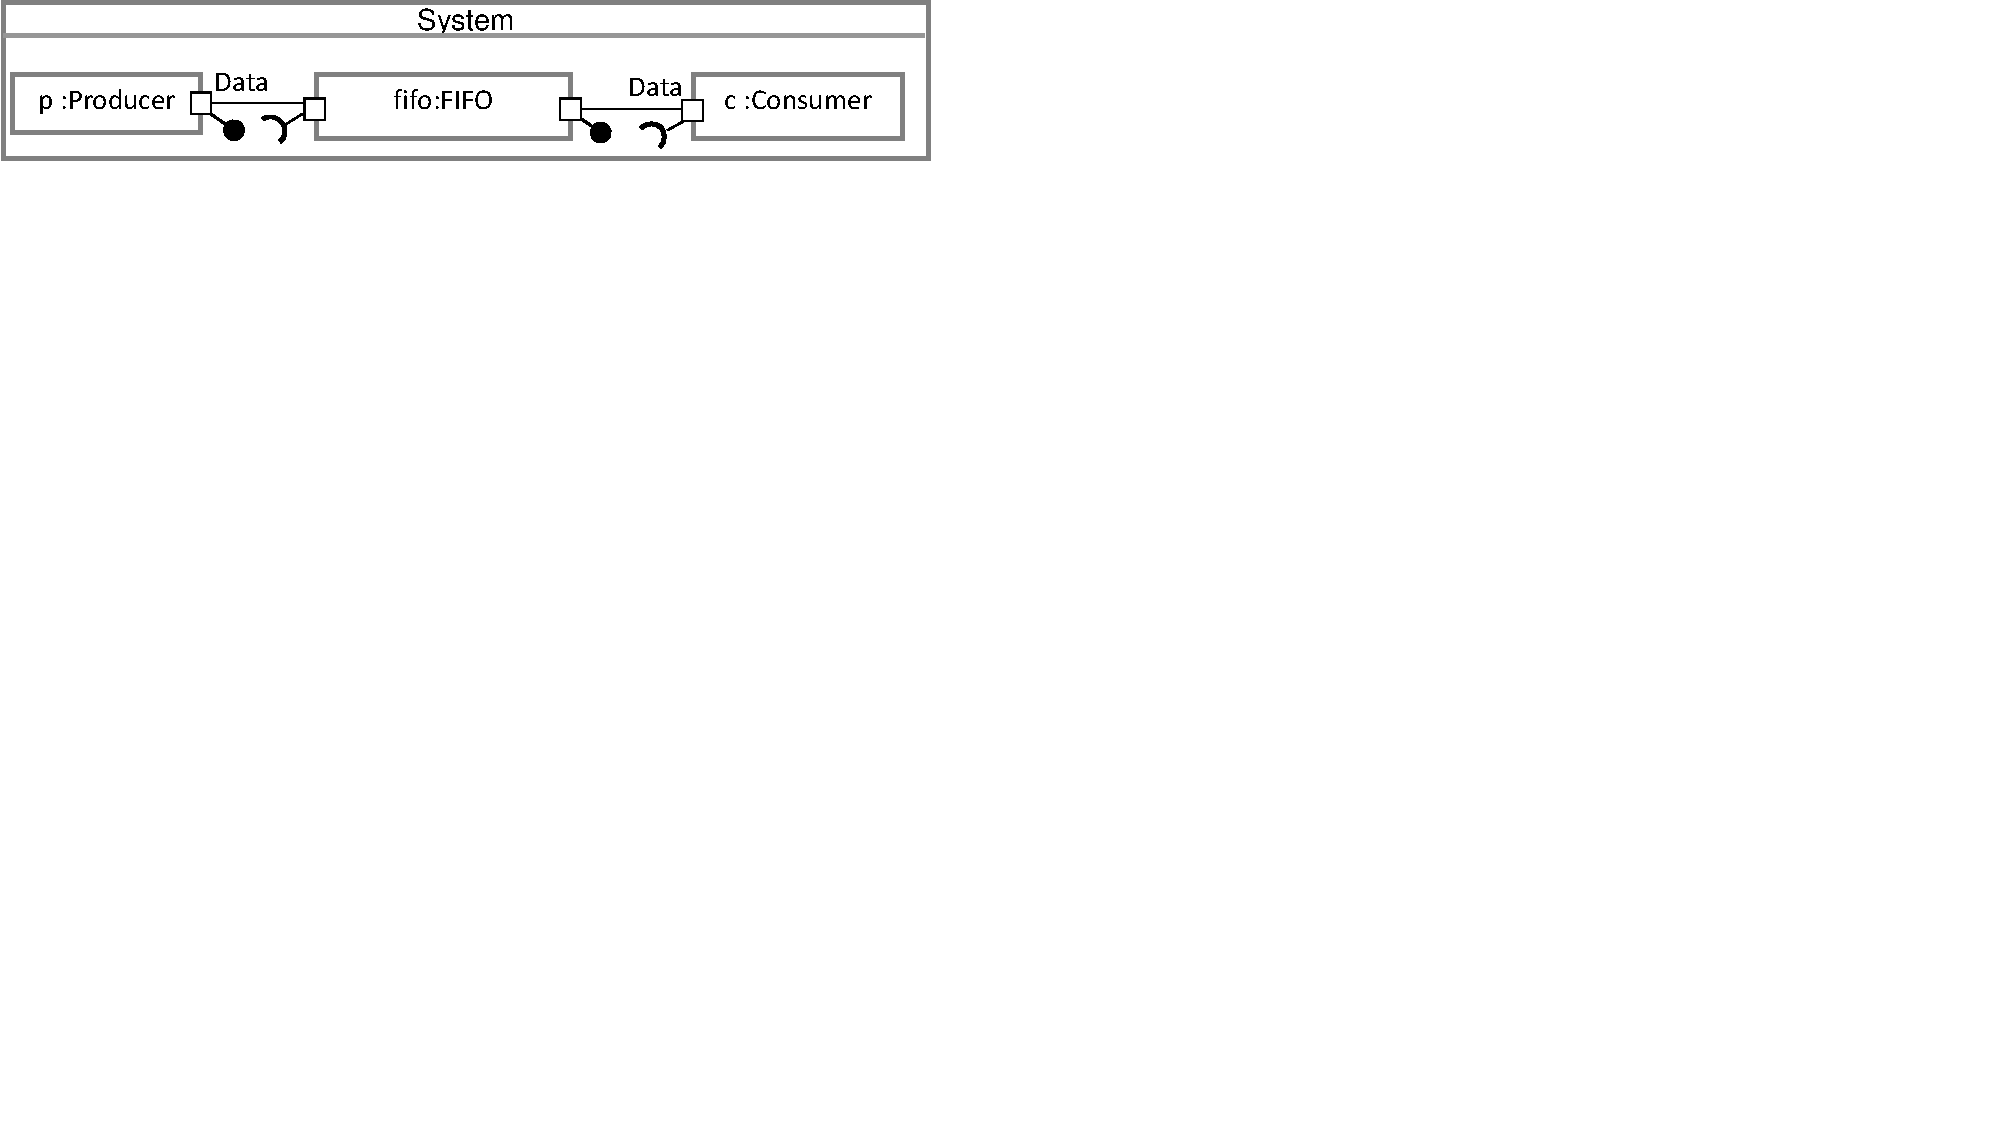
\includegraphics[clip, trim=0cm 16.3cm 17.6cm 0cm, width=\columnwidth]{figures/dataportexample.pdf}
	\caption{Component-based architecture example with data port} 
	\label{fig:dataportexample}
\end{comment}


\begin{minipage}{0.95\columnwidth}
	\lstinputlisting[language=C++, caption={System using data ports}, label=lst:dataport,frame=f]{code/dataport.cpp}
\end{minipage} 

In system implementation, the producer provides data items to the fifo via the port \ttt{pProvideData} by calling \ttt{pProvideData->sendSignal(item)} as an object-oriented way.
In case that the behavior of the component is described by a state machine, the \ttt{sendSignal} method will fire a signal event in order for the state machine to handle it.


\vskip 0.1cm
\tb{Discussion:}
Compared to other code generation approaches, the philosophy of XSeparation is different.
Usually, a code generation approach refines the architecture model at high level of abstraction to the code through a chain of transformations.
Although the latter help to modularize the code generation process, hence make it easy to implement, the traceability from the code back to the model becomes very hard because the abstraction gap degree increases at each transformation.

XSeparation generates code at an intermediate abstraction level. 
Fig. \ref{fig:transformationchain} shows how different XSeparation is from the other approaches.
We argue that synchronization of model and code at different abstraction is a very hard problem, even impossible because component concepts such as part, port, and connectors are not directly mapped to object-oriented code. 
To deal with it, XSeparation proposes to preserve the abstraction level of these concepts by representing and introducing additional equivalent classes/constructs to object-oriented code as shown in the example in Listing \ref{lst:architectureprescribed}.
Other modeling concepts such as properties and operations are generated to code using a trivial mapping used by many industrial code generation tools such as Rhapsody.

Although introducing additional constructs is not really new when compared to Archface \cite{ubayashi2010archface} and \cite{aldrich2002archjava}, these approaches are very language-specific.
XSeparation is, on the other hand, purely object-oriented, hence better suitable to object-programmers. 
Furthermore, the programmers can write interaction code between components (Listing \ref{lst:producerinteraction}) by the way, which fully profits advantages of familiar integrated development environments such as Eclipse without having to install any additional tools/plug-ins.  

%should be moved to related work???
XSeparation and the \ttt{1.x-way mapping deep separation} approach are similar in the philosophy of separating completely \tb{Component structure-prescribed code} and \tb{User-filled skeleton code} in different constructs, the two approaches are fundamentally not the same. 
\ttt{Deep separation} ignores modifications made to the architecture at the code level, hence much assumes that the programmers are not interested in modifying architecture.
It, however, contradicts with the need pointed out by R. N. Taylor et al. \cite{Taylor:2007:SDA:1253532.1254721} as previously discussed. 

XSeparation, 
%on the other hand, puts the architecture information in code at the right abstraction level with appropriate additional constructs.
%By this way, XSeparation, 
%compared to \ttt{deep separation}, 
gives programmers the ability for not only understanding but also modifying the architecture at the code level.
Because the abstraction level of component modeling concepts are preserved, XSeparation enables the reflection of modifications made in code to the model.

\begin{figure}
	\centering
	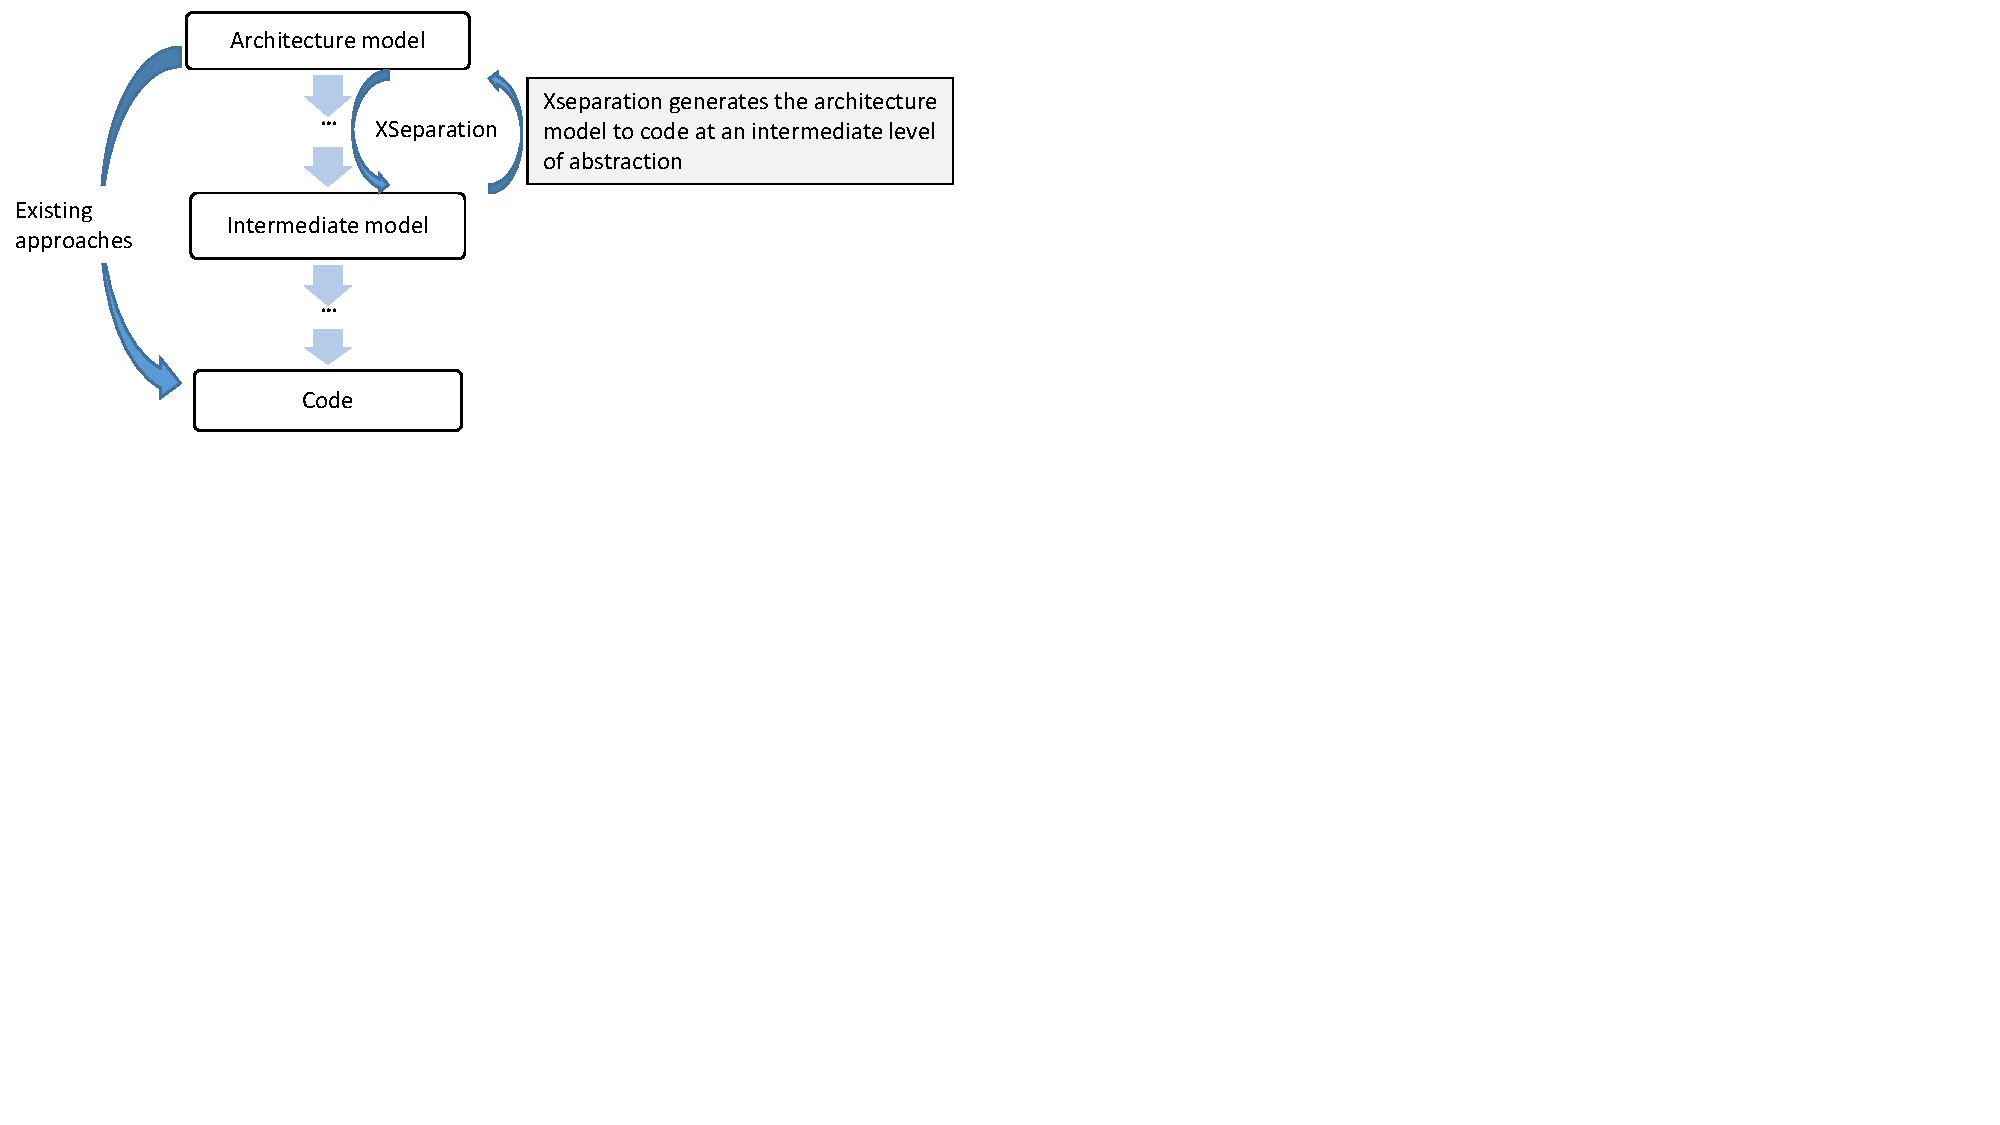
\includegraphics[clip, trim=0cm 11.3cm 17.6cm 0cm, width=\columnwidth]{figures/transformationchain.pdf}
	\caption{Comparison of XSeparation with other code generation approaches} 
	\label{fig:transformationchain}
\end{figure}




We have presented how XSeparation works for the architecture structure.
In the next section, XSeparation for the architecture behavior described by UML State Machines will be detailed.